% declare what packages you use:
\documentclass[12pt]{article}
\usepackage[utf8]{inputenc}
\usepackage{amsmath}
\usepackage{amssymb}
\usepackage{amsthm}
\usepackage{enumitem}
\usepackage{mathtools}
\usepackage[letterpaper]{geometry}
\geometry{margin=0.8in}
\usepackage{hyperref}

% The title of the report
\title{Proof Activity Report}
% Write your name in author
\author{Rita Qifan Yang }
% Course code and date
\date{Comp251, Winter 2023}



\begin{document}
\maketitle

% Report the first claim you will prove here
\section*{Claim 1}
Inserting a node $x$ into a heap takes $O(logn)$ time. 


% Report the proof of the claim here
\section*{Proof}
The heap data structure is an array object that can be viewed as a nearly complete binary tree \cite{cormen2009introduction}. There are two kinds of binary heaps, this proof will use a max-heap, where the biggest element is at the root. A min-heap can be used for proof in the exact same way, but with an opposite heap property where the smallest element is at the root. This proof is paraphrased from Cormen, Leiserson, Rivest, and Stein, \textit{Introduction to Algorithms}, \cite{cormen2009introduction}, page 128 - 144. 
\begin{proof}
There are $2$ components of inserting a node into the heap data structure that we can reason about individually.
\begin{enumerate}
    \item \textsc{Heap-Increase-Key(A,i,key)}
    This method takes a new key and an index, if the key is smaller than the key at the index, method returns error, otherwise, it keeps going up and exchange the key with their parents. 
    \item \textsc{Max-Heap-Insert(A,key)} 
    It takes a key and and an array $A$ and first expands the maxheap by adding to the tree a new leaf whose key is $ - \infty$. Then it calls \textsc{Heap-Increase(A,i,key)} to set the key of this new node to its correct value and maintain the max-heap property.
    
\end{enumerate}
The running time of \textsc{Heap-Increase-Key(A,i,key)} on an $n-$ element heap is $O(logn)$, since the path from node to the root as length $O(logn)$. The expansion and leaf insertion in \textsc{Max-Heap-Insert(A,key)} takes $O(1)$ each, and it calls  \textsc{Heap-Increase(A,i,key)} once. Therefore, the total running time is $O(1)$ + $O(1)$ + $O(log n)$ = $O(logn)$. 

\end{proof}

% Report the summary of the proof here
\section*{Proof Summary}
We argue the running time of each of the two main components in the algorithm. Expanding the array size and adding a new key takes constant time, switching the new node with its parents repeatedly (if it is bigger than the parent) in the worst case will take us all the way until the root node. Therefore in the worst case, it has to be switched for the length of the path from the bottom to the top. Since the max heap property holds, it can stop when the parent is larger(since all parents of the parent is larger than or equal to the parent), therefore we only stop once at each level of the tree. The worst case time complexity will be the height of the this nearly complete binary tree.

% Report the algorithm and java code here, including any relevant figures
\section*{Algorithm}
Below is the Java code for the Insertion method in a max-heap. I created two methods needed for the algorithm. This includes the \textsc{Heap-Increase-Key(A,i,key)} (Figure 1), \textsc{Max-Heap-Insert(A,key)}(Figure 2). 

I time the execution of the insertion by counting the number of levels that the node traversed up to the root. I increase the size of the heap by $10$ for each new instance and repeat $2000$ times. In total, I timed the execution of heaps size up to $n=20000$. The execution time is reported in number of steps in the while loop in \textsc{Heap-Increase-Key(A,i,key)} when we try to insert a new key with a value bigger than the root. The plot below (Figure 5) shows the execution time as a function of the number of vertices, $n$. We expect the execution time to be logarithmic in $log_{2}{n}$, and to be a upper bound. The graph confirms this claim. It can be closely modelled by the logarithmic function of $log_{2}{n}$ shown. 

The methods \textsc{Max-Heapify(A,i)}, and \textsc {Build-Max-Heap(A)} (for building and maintaining the heap) are not needed in this variation of the algorithm as the initial array holds max-heap property. However, they are necessary in order to generate max heaps in order to time the execution (figure 4), they can both be found in \texttt{ComplexityProof.java}.



\begin{figure}[h]
  \centering
    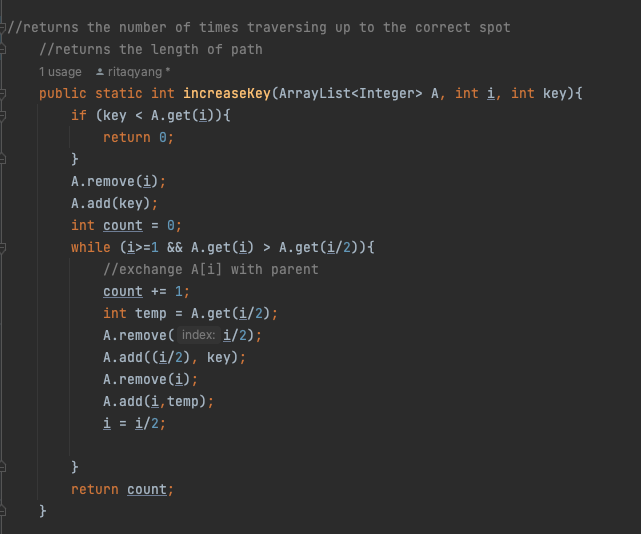
\includegraphics[scale=.5]{COMP251 Sample Report/figures/inceaseKey.png}
        \caption{Method increaseKey from \texttt{ComplexityProof.java}.}
\end{figure}

\begin{figure}[h]
  \centering
    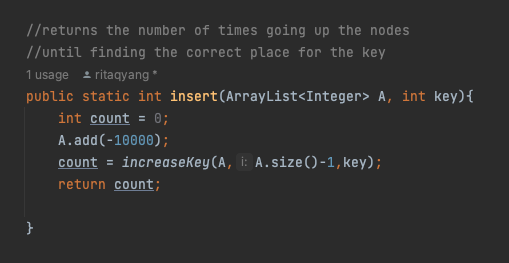
\includegraphics[scale=.8]{COMP251 Sample Report/figures/insert.png}
        \caption{Method insert from \texttt{ComplexityProof.java}.}
\end{figure}

\begin{figure}[h]
  \centering
    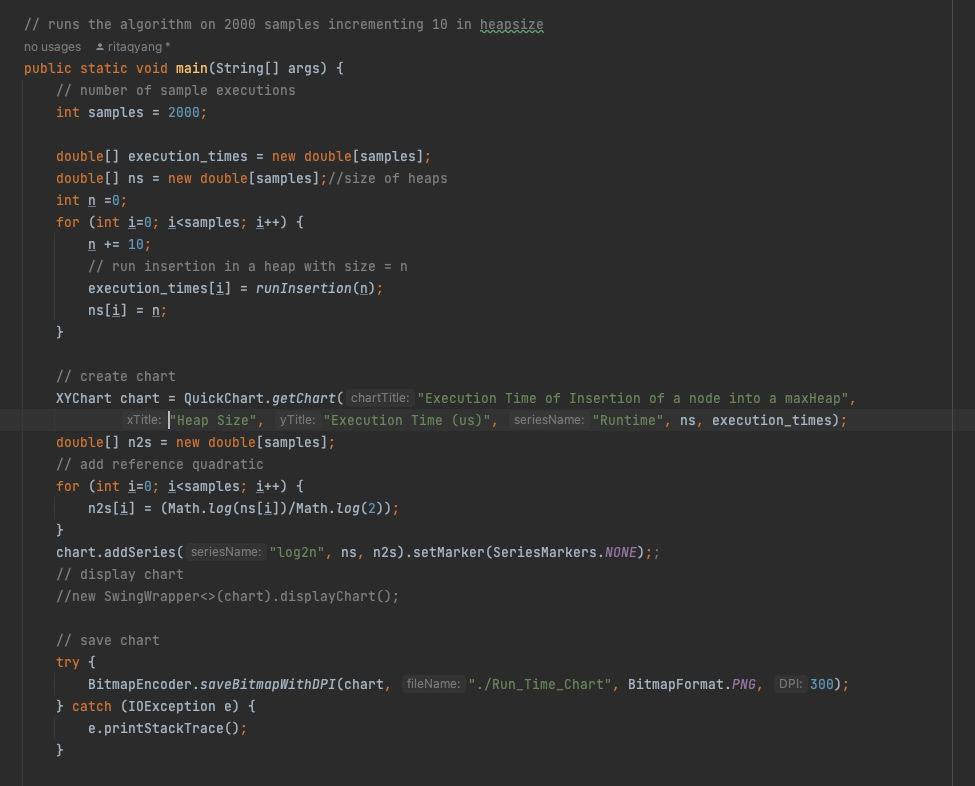
\includegraphics[scale=.5]{COMP251 Sample Report/figures/sample.png}
        \caption{Main Method generating the samples and the graph from \texttt{ComplexityProof.java}.}
\end{figure}

\begin{figure}[h]
  \centering
    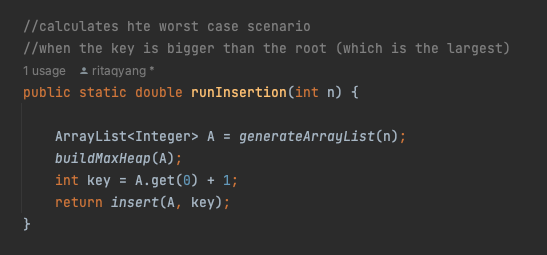
\includegraphics[scale=.7]{COMP251 Sample Report/figures/runinsertion.png}
        \caption{Method runInsertion from \texttt{ComplexityProof.java}.}
\end{figure}

\begin{figure}[h]
  \centering
    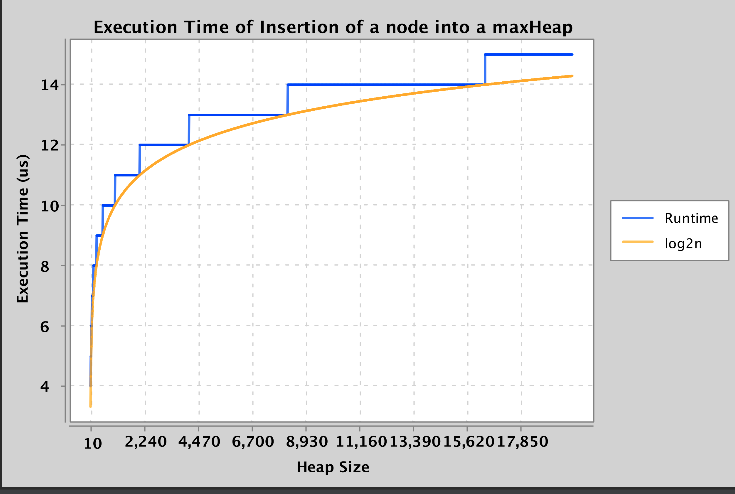
\includegraphics[scale=.5]{COMP251 Sample Report/figures/time complexity.png}
        \caption{ Inserting a node into a binary heap takes $O(logn)$ time. }
\end{figure}

\clearpage
% Report the real world application here
\section*{Real World Application} 
Heaps can be used to implement priority queues, that can be useful in prioritizing customers waiting to pay in a supermarket, stock options on stock exchange websites, and hospitals prioritizing patients based on how urgent their problem is, etc. One way to model the customer in a supermarket problem is to assign each person in the line a node where the value corresponds with the amount of time the person has stood in line. People who stood in line for the longest will have a larger key value. The root of the heap will be the person that has paid for their items, their node will then be extracted from the heap, and then we can MaxHeapify to get the new line\cite{bri}. In a similar hospital example, the insertion will be important as a new patient can come in the line with very urgent medical issues than people who have waited for longer. So being able to quickly insert patients into the right spots in the priority queue allows the emergency room / hospital to function more effectively\cite{geeks}.



\newpage
% Report the second claim you will prove here
\section*{Claim 2}
The Heapsort Algorithm: Argue the correctness of \textsc{heapsort} using the following loop invariant: At the start of each iteration of the for loop of the subarray $A[ 1...i ]$ is a maxheap containing the $i$ smallest elements of $A[1...i]$, and the subarray $A[i+1...n]$ contains the $n-i$ largest elements of $A[1...n]$, sorted. 


\section*{Proof}
% Report the proof of the claim here
This proof is paraphrased from Cormen, Leiserson, Rivest, and Stein, \textit{Introduction to Algorithms}, \cite{cormen2009introduction}
\begin{proof}
The Heapsort Algorithm contains $3$ components. To prove the correctness of Heapsort using the given loop invariant, we first lay out the algorithm structure, then we discuss $3$ main stages of iteration: \textsc{Initialization},
\textsc{Maintenance},and \textsc{Termination}. 
\begin{enumerate}
  
    \item \textsc{Max-Heapify(A,i)}
    This function is an important subroutine for manipulating max-heaps, it takes an array $A$ and and index for the node $i$. When the function is called, it is assumed that the binary trees rooted on the left and right side of the node $i$ are already max-heaps, but that $A[i]$ may be smaller than its children, thus violating the max-heap property. The function allows $A[i]$ to "float down" in the max heap so that the subtree with root at $i$ follows the max-heap property.
    \item \textsc{Build-Max-Heap(A)} 
    We can construct the heap using an "bottom-up" approach. Assume the size of the array $A$ is $n$, we iterate from $n/2$ down to  $1$ and call \textsc{Max-Heapify(A,i)} at each iteration. 
    \item \textsc{HeapSort(A)} starts by using \textsc{Build-Max-Heap} to build a max heap on the input array $A$. Since the maxium element is at the root, it can be put to the final position by exchanging with $A[n]$. Then we discard node $n$ by decresing the heap size and we try restore the max-heap property by calling \textsc{MAx-heapify} once on the new root.
\end{enumerate}



\textsc{Initialization}:  Prior to the first iteration, $i = n$, $A[1...n]$ is a max heap and the second subarray is empty. 

\textsc{Maintenance}: To see that each iteration maintains the loop invariant, observe that the largest node $A[0]$ will switch place with $A[i]$, then heap size decrease by one, so the root joins the second subarray that is now $A[i...n]$. Since its given that the $A[i+1...n]$ contains the $n-i$ largest elements,  the root node is the smallest of $A[i...n]$ and biggest in $A[1...i-1]$ because of the max heap property, so the loop invariant maintains. Then we find the correct place for the new root to restore the max heap property of $A[1...i-1]$. Decrementing the i in the for loop update reestablishes the loop invariant for the next iteration. 

\textsc{Termination}: At termination, $i = 2$. By the loop invariant, the first two nodes holds max heap property, so the first node exchange places with the second node, heap size decreases to 1, and now we have a max heap of size $1$, and $A[2...n]$ is the sorted list of the biggest elements in $A$. 

\end{proof}

\section*{Proof summary}
The real meat of the proof is the max-heap property. Since all parents are always bigger than or equal to their children, when the max node is removed from the root each time, the remaining heap is very close to satisfying the max-heap property, we only need to find the correct place for the new root and max-heap property can be restored. Therefore, we have the first subarray that is a max-heap at the start of each for loop after we restore the max-heap property in the prior iteration. And largest elements (who are nodes that got removed from the root) are sorted in the second subarray because the they are removed in order to the back at each iteration as the root nodes. Below is a helpful demonstration of the algorithm (figure 6).  

\begin{figure}[h]
  \centering
    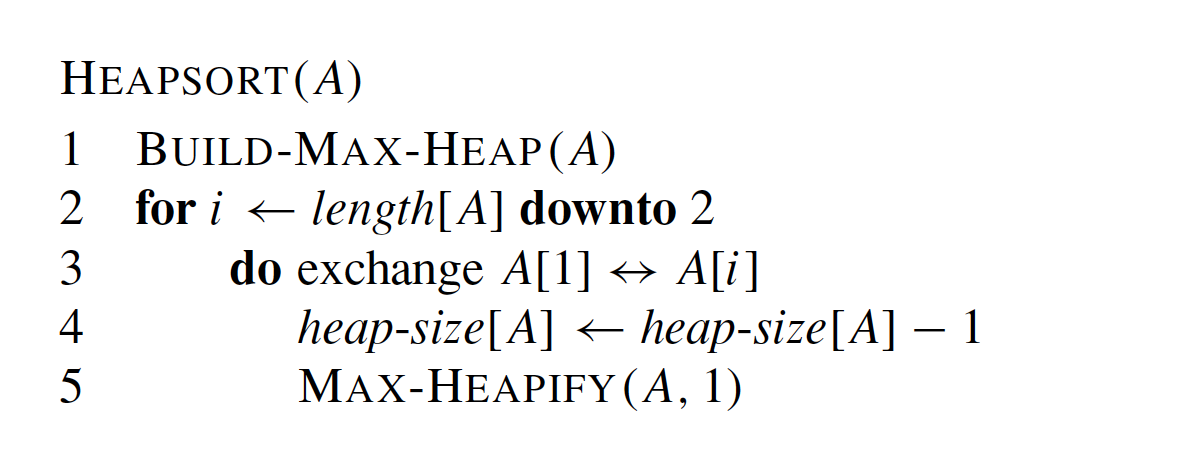
\includegraphics[scale=.5]{COMP251 Sample Report/figures/Heapsort.png}
        \caption{Heapsort Algorithm from \cite{cormen2009introduction}}
\end{figure}

\section*{Algorithm}
Below is the Java code for the Heapsort algorithm. The implementation required is a \textsc{Max-Heapify(A,i)} method (figure 7), a \textsc{Build-Max-Heap(A)} method (Figure 8), a \textsc{HeapSort(A)} method (figure 9), and a file which contains the algorithm, main function and several helper functions for the test cases.

The main function executes the algorithm on three cases. And the heapSort method prints information at the start of each iteration. The output of the algorithm on the three test cases is shown in Figure 10, 11, and 12.

First is a general case. We use the textbook example $\{16,14,10,8,7,9,3,2,4,1\}$ as shown in figure 10. A helpful visualization can be found in figure 11. The first edge case is when multiple nodes are equal.We used $\{16,16,15,15,14,10,8,8,7,9,3,2,4,1,1,1\}$ (figure 12); Finally, the second edge case is when all but one node are equal, we used $\{16,16,16,16,16,16,16,16,16,8\}$ (figure 13).

For each case, we examine every iteration from before initiation to after termination. Each step are shown on the console output. We can see that in every iteration, the first array maintains max-heap property where every child is less than or equal to the parent, the second is a sorted list of the biggest $n-i$ elements in the array. 

\clearpage

\begin{figure}[h]
  \centering
    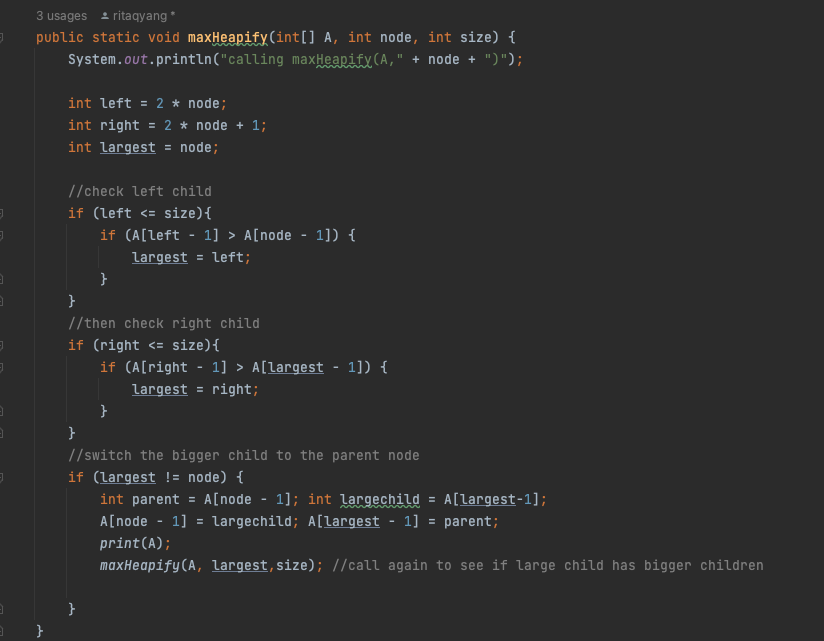
\includegraphics[scale=.5]{COMP251 Sample Report/figures/MaxHeapify.png}
    \caption{Method maxHeapify from \texttt{Heapsort.java}.}
\end{figure}

\begin{figure}[h]
  \centering
    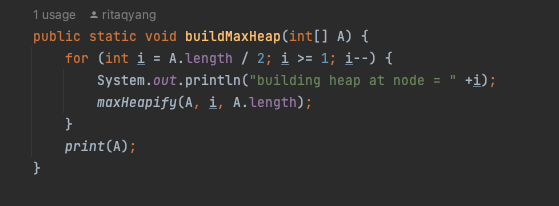
\includegraphics[scale=.7]{COMP251 Sample Report/figures/buildMaxHeap.png}
    \caption{Method buildMaxHeap from \texttt{Heapsort.java}.}
\end{figure}

\begin{figure}[h]
  \centering
    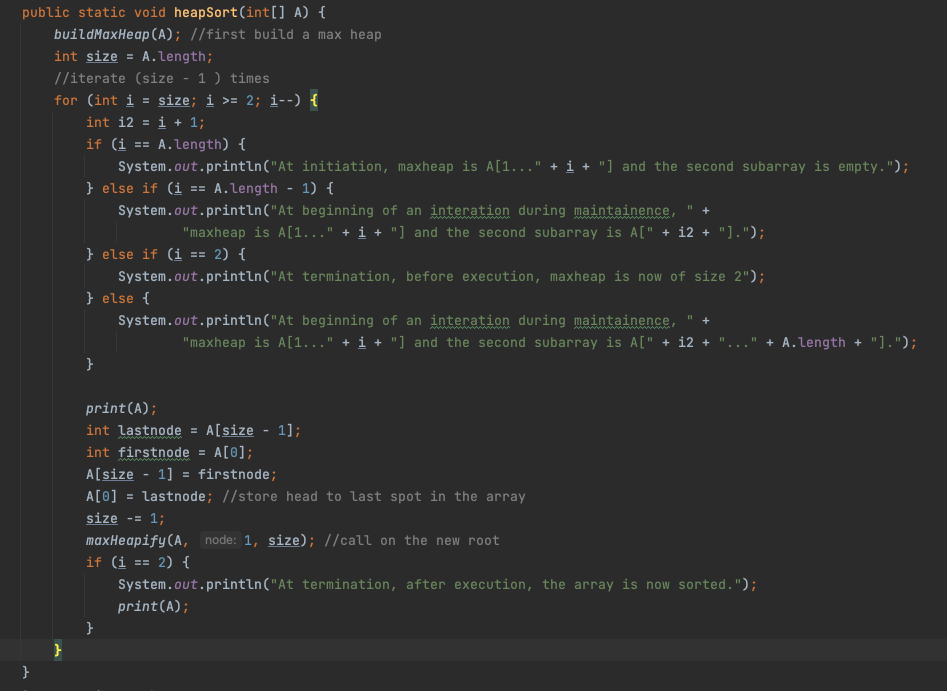
\includegraphics[scale=.4]{COMP251 Sample Report/figures/sort.png}
    \caption{Method heapSort from \texttt{Heapsort.java}.}
\end{figure}


\begin{figure}[h]
    \centering
    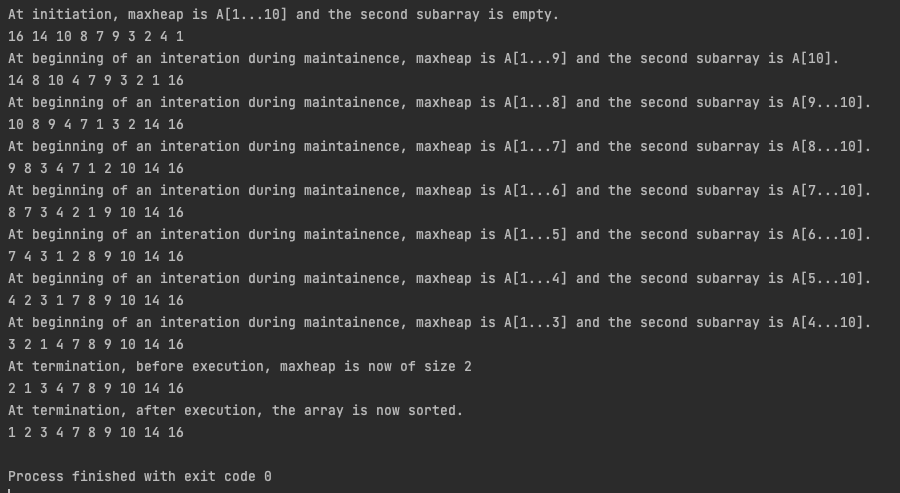
\includegraphics[scale=.4]{COMP251 Sample Report/figures/console.png}
    \caption{Console output of general case (textbook example) from \texttt{Heapsort.java}.}
\end{figure}
\begin{figure}[h]
    \centering
    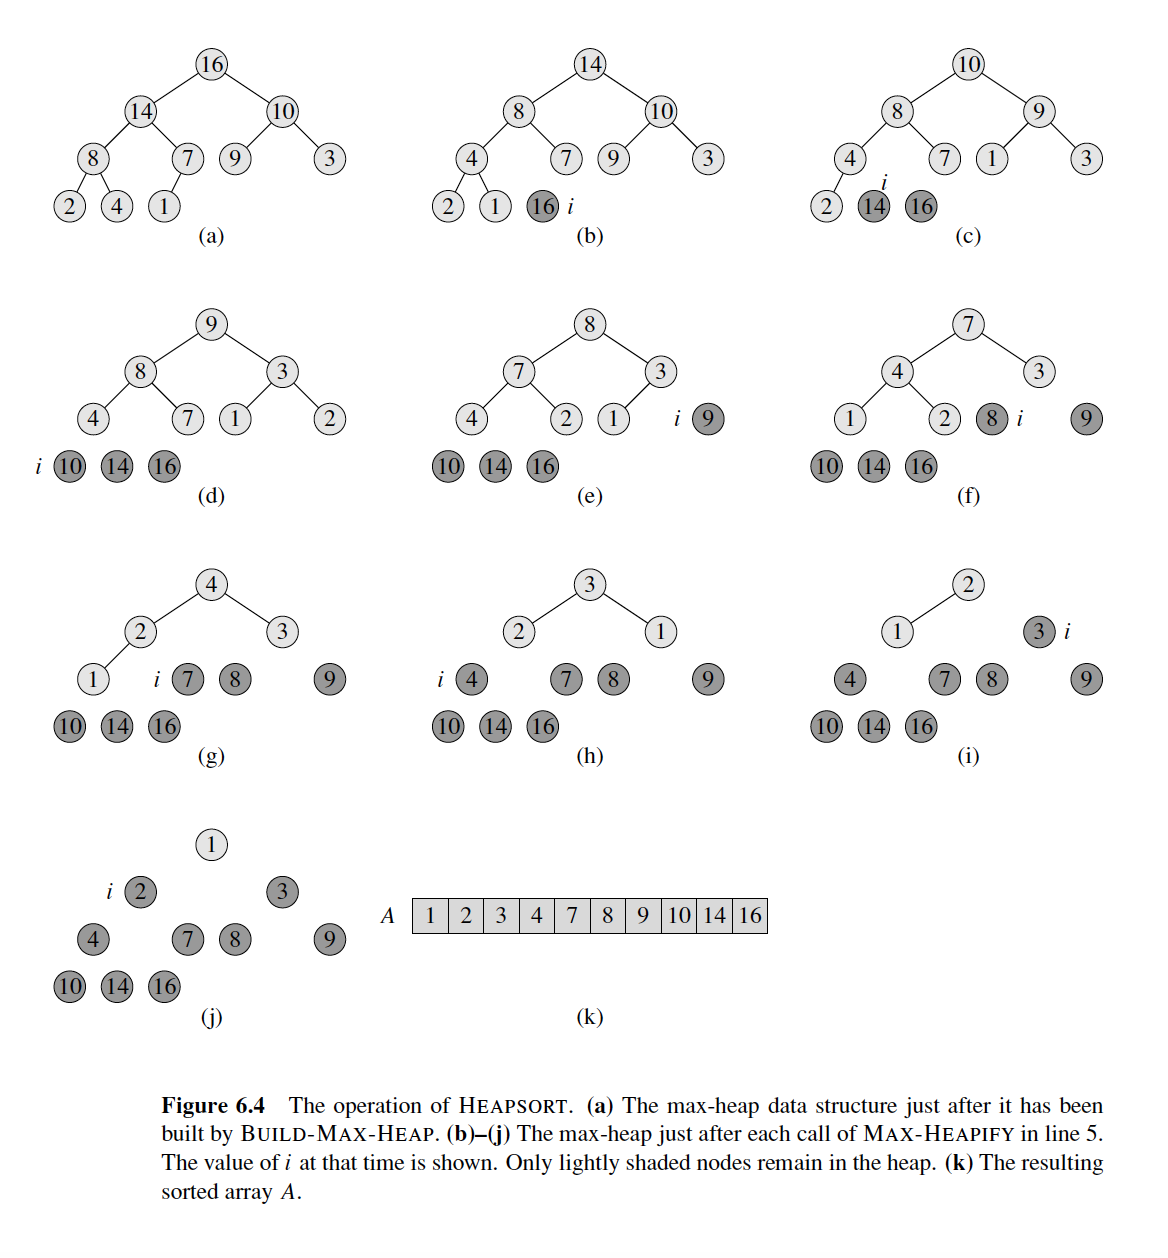
\includegraphics[scale=.5]{COMP251 Sample Report/figures/Heapsort Corretness example.png}
    \caption{Visualization of the textbook example from Cormen, Leiserson, Rivest, and Stein, \textit{Introduction to Algorithms}, \cite{cormen2009introduction}, page 137}
\end{figure}
\begin{figure}[h]
    \centering
    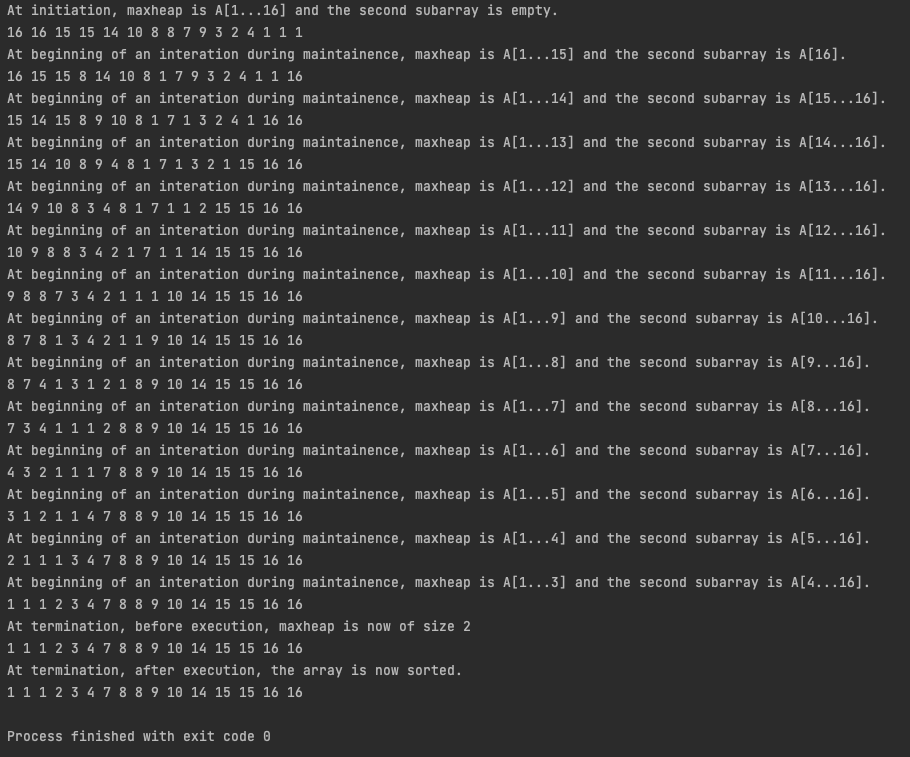
\includegraphics[scale=.4]{COMP251 Sample Report/figures/edge4.png}
    \caption{Console output of edge case where some nodes are equal from \texttt{Heapsort.java}.}
\end{figure}

\begin{figure}[h]
    \centering
    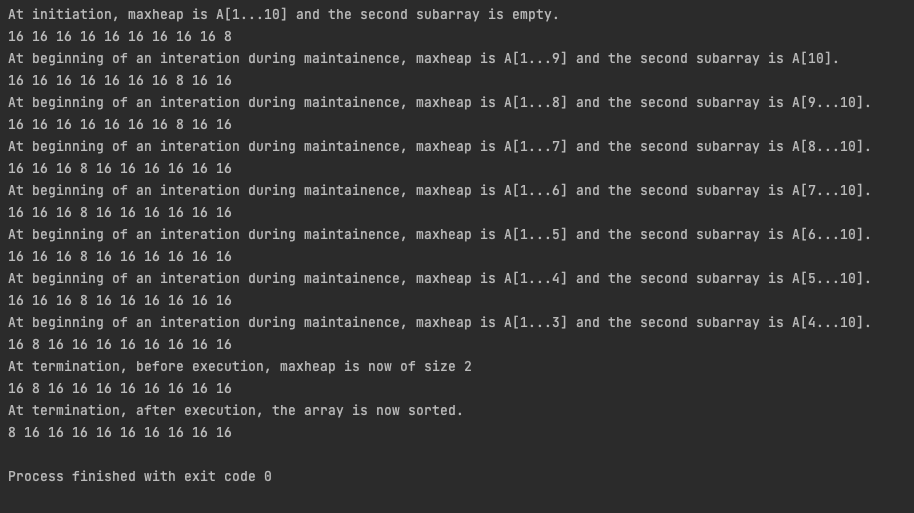
\includegraphics[scale=.4]{COMP251 Sample Report/figures/egde5.png}
    \caption{Console output of edge case where all but one node are equal \texttt{Heapsort.java}.}
\end{figure}



\clearpage
\section*{Real World Application}

\textsc{Heapsort} can be very useful for other algorithms. Firstly, Huffman coding algorithm used in data compression uses a priority queue implemented as a min-heap to build a Huffman tree. Huffman code creates a queue consisting of each unique character and sorts in ascending order of their frequencies. Extracting minimum frequency from the priority queue takes place $2 \cdot (n-1)$ times and each time takes $O(logn)$ time, which is optimized by \textsc{Heapsort}\cite{huffman}. Secondly, \textsc{Heapsort} is also used in external sorting algorithms and processes chunks of data in a priority queue to sort large datasets that do not fit into memory. In addition, \textsc{Heapsort} can be used in load balancing algorithms to find the smallest load and therefore effectively distribute tasks and requests to servers \cite{geeks}. 





\clearpage
% Creates bibliography (if using bibtex)
\bibliographystyle{plain}
\bibliography{myref.bib}

\end{document}
